\documentclass{beamer}
\usepackage{beamerthemesplit}
\usepackage{subfig}
\usepackage{amssymb,amsmath,mathtools}
\usepackage{amsfonts,booktabs}
\usepackage{lmodern,textcomp}
\usepackage{color}
\usepackage{tikz}
\usepackage{natbib}
\usepackage{multicol}
\usepackage{ctex}
\usepackage[level]{datetime}
\usepackage{listings}


\usetheme{Warsaw}
\newdateformat{ukdate}{\monthname[\THEMONTH] \ordinaldate{\THEDAY} , \THEYEAR}
\lstset{
 columns=fixed,       
 numbers=left,                                        % 在左侧显示行号
 numberstyle=\tiny\color{gray},                       % 设定行号格式
 frame=none,                                          % 不显示背景边框
 backgroundcolor=\color[RGB]{245,245,244},            % 设定背景颜色
 keywordstyle=\color[RGB]{40,40,255},                 % 设定关键字颜色
 numberstyle=\footnotesize\color{darkgray},           
 commentstyle=\it\color[RGB]{0,96,96},                % 设置代码注释的格式
 stringstyle=\rmfamily\slshape\color[RGB]{128,0,0},   % 设置字符串格式
 showstringspaces=false,                              % 不显示字符串中的空格
 language=c++,                                        % 设置语言
}


\title{基于生成式先验的人像视频编辑}
\author{汪兆辰}
\date{\ukdate\today}

\begin{document}

\begin{frame}
    \titlepage
\end{frame}

\section{近期进展}

\begin{frame}
    \frametitle{上次的问题}
    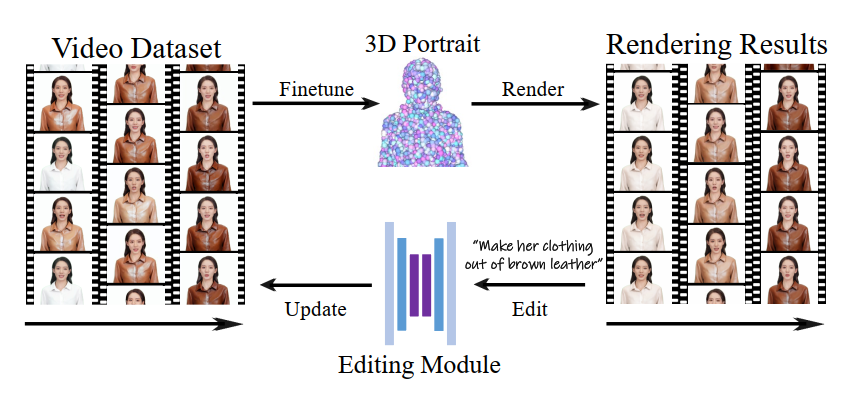
\includegraphics[width=\textwidth]{pic1.png}
\end{frame}

\begin{frame}
    \frametitle{上次的问题}
    \begin{itemize}
        \item 在每个epoch中只抽100帧左右,因此时间开销在30min左右,可以接受
        \item 但在数学上并不能证明该更新过程是收敛的,事实上在实验上确实有许多不收敛到预期结果的情况,主要发生在打光和换衣两个任务中
    \end{itemize}
\end{frame}

\begin{frame}
    \frametitle{近期进展}
    \begin{itemize}
        \item 初步制定了需求分析,近期在尝试修改神绘数字人网站的代码,在网站的UI设计,数据库设计等方面将以该网站为基础
        \item 算法方面在配置环境方面遇到一些问题,正在解决
    \end{itemize}
\end{frame}

\section{问题}

\begin{frame}
    \frametitle{问题}
    \begin{itemize}
        \item 在本地部署portraitgen代码时由于开发环境不同,每一步都遇到问题
        \item 换到服务器上按照README重新部署的过程中,仍然遇到bash脚本跑不通的问题,正在逐个解决
    \end{itemize}
\end{frame}

\section{编程提高}
\begin{frame}
    \frametitle{每日一题}
    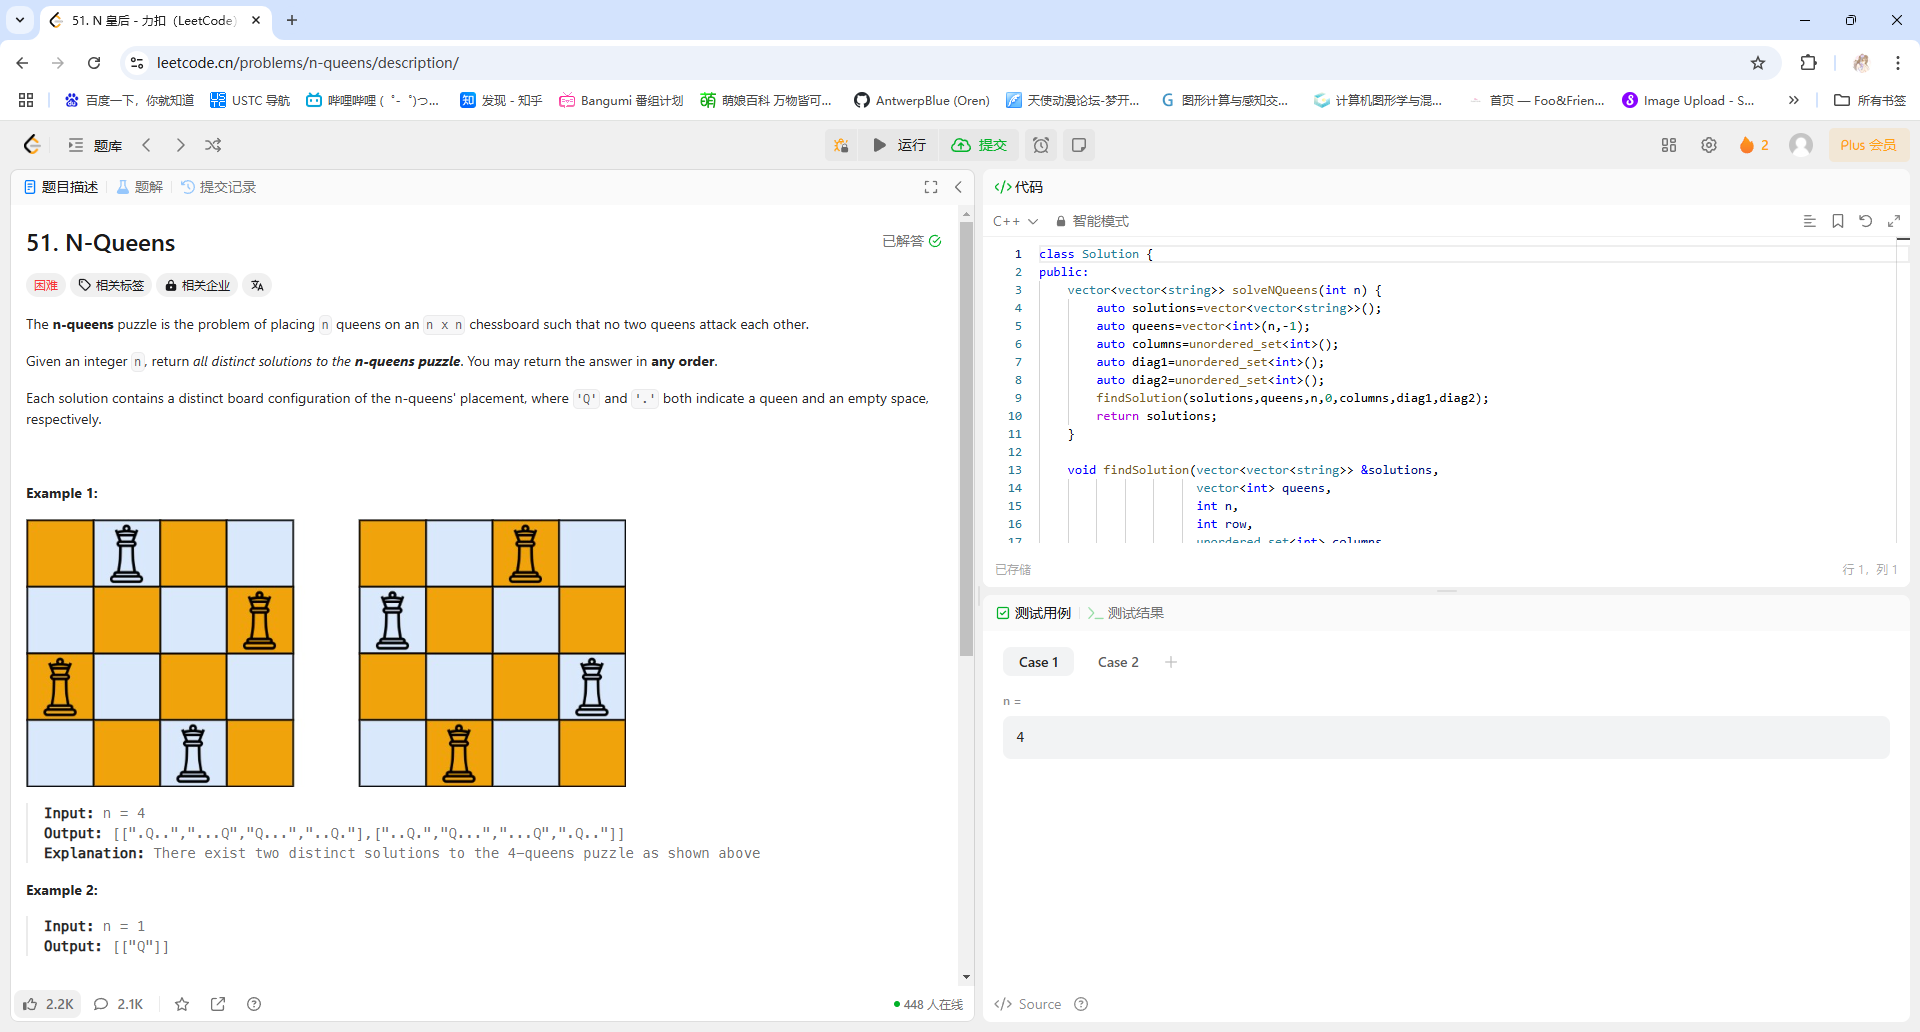
\includegraphics[width=\textwidth]{pic2.png}
\end{frame}

\begin{frame}
    \frametitle{热题题单}
    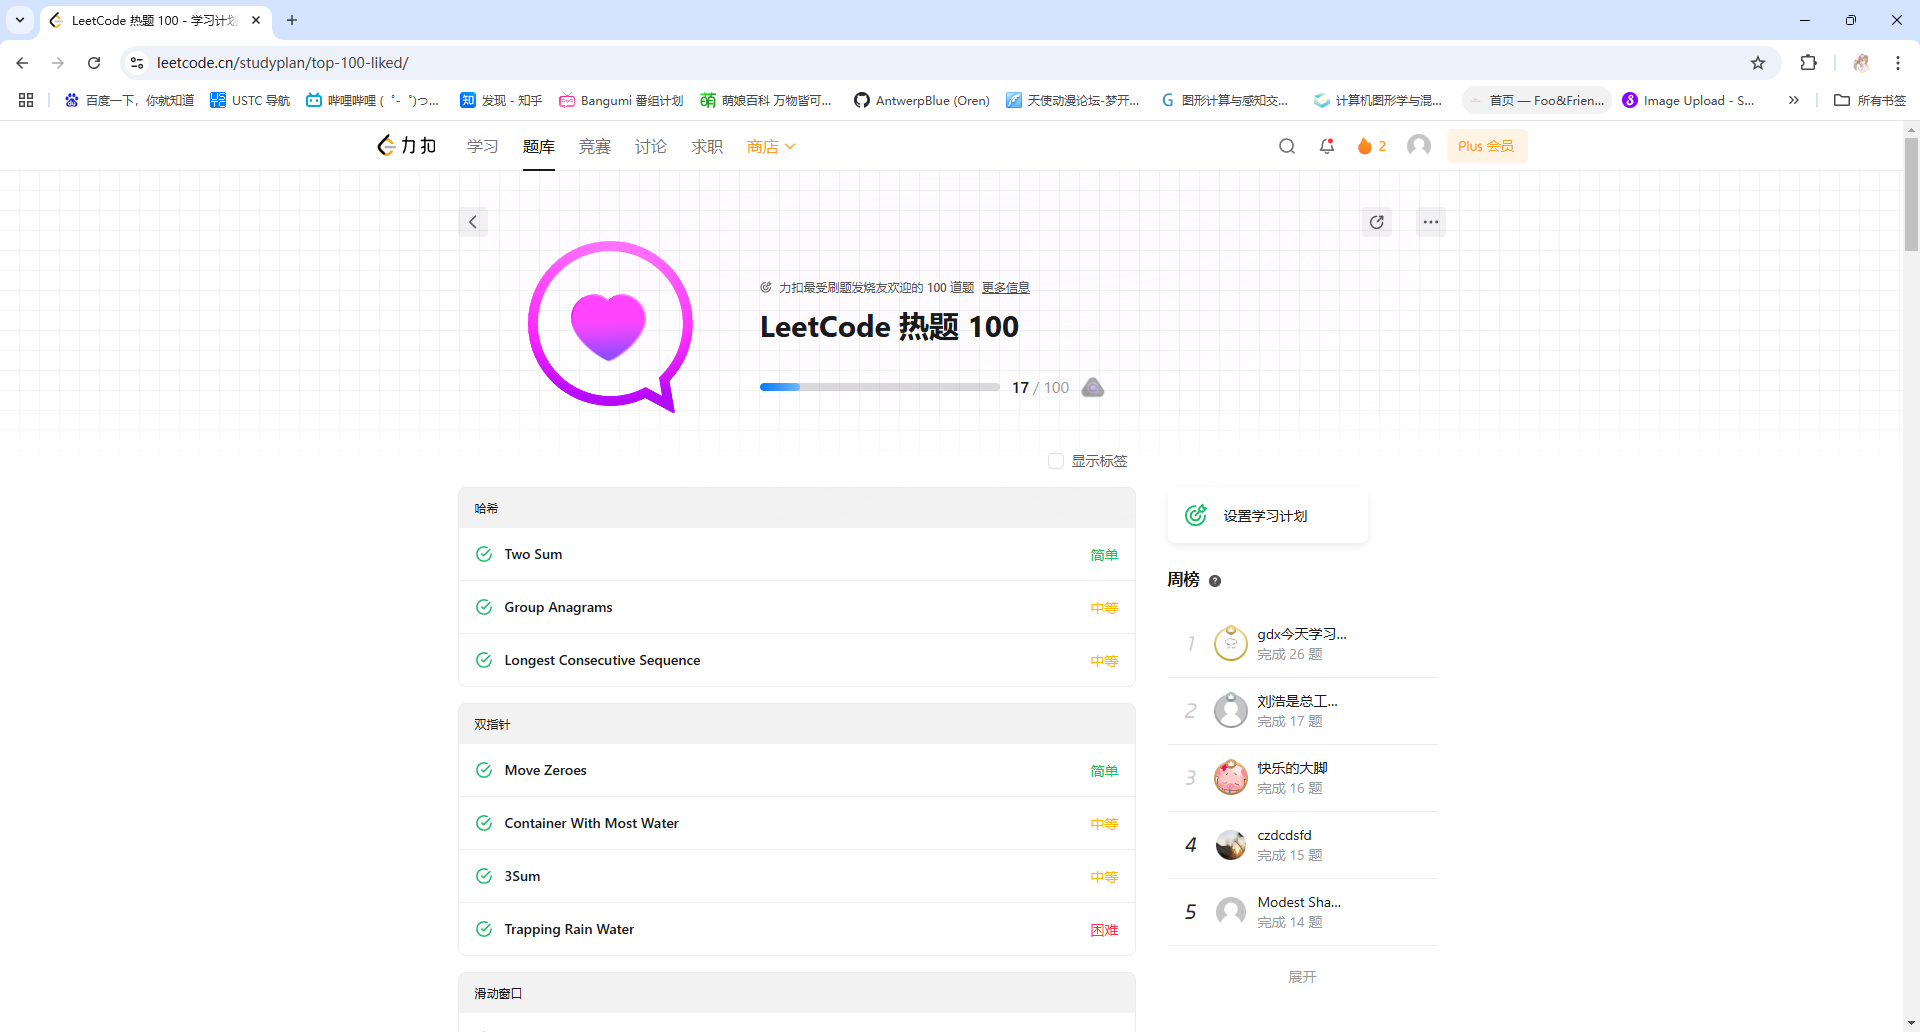
\includegraphics[width=\textwidth]{pic3.png}
\end{frame}


\end{document}